\documentclass{article}
\usepackage{graphicx}
\usepackage[margin=1.5cm]{geometry}
\usepackage{amsmath}

\begin{document}

\title{Thursday Reading Assessment: Unit 4, Magnetic Induction}
\author{Prof. Jordan C. Hanson}

\maketitle

\section{Memory Bank}

\begin{itemize}
\item $\epsilon = -N \Delta \phi_m /\Delta t$ ... Faraday's Law
\item $\phi_m = \vec{B} \cdot \vec{A}$ ... Definition of magnetic flux
\end{itemize}

\section{Faraday's Law}

\begin{enumerate}
\item Suppose a uniform B-field of 0.01 T made an angle of 45 degrees with an area of 0.1 m$^2$.  (a) Calculate $\phi_m$, the magnetic flux. (b) Suppose the B-field drops to 0 T in 10 ms.  What is $\Delta \phi_m / \Delta t$? \\ \vspace{2cm}
\item Consider Fig. \ref{fig:current}.  Suppose a constant current $I$ is flowing through a rigid rod that hangs vertically from flexible leads, and suddenly a B-field appears within the rectangle formed by the rod and leads.  \textbf{The B-field is into the page.}  The vertical portion containing the battery and resistor is also rigid.  The mass $m$ and length $L$ of the rod have been chosen such that $I = \lambda g / B$, where $\lambda = m/L$.  (a) What is the magnitude of the Lorentz force, in terms of the variables given?  (b) What is the magnitude of the weight force, in terms of the variables given?  (c)  Show that if these two forces are equal, $I = \lambda g / B$. (d) Given that the net force is 0, the rod can rise at constant velocity.  What will happen to $\phi_m$ if the rod rises?  What does this imply about $\epsilon$? 
\end{enumerate}
\begin{figure}
\centering
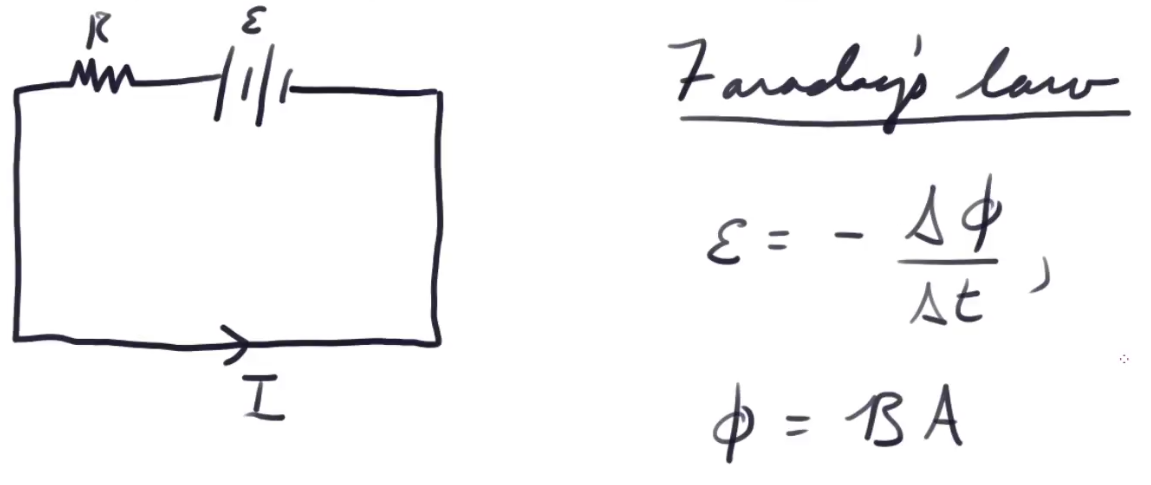
\includegraphics[width=0.5\textwidth]{current.png}
\caption{\label{fig:current} A current-carrying rod of length L hangs vertically in a B-field that turns on suddenly and \textit{is in to the page}.  The rod cannot change length, but the vertical leads are flexible and can change length.}
\end{figure}
\end{document}
